
\chapter{Introduction}
\label{chap:introduction}
\pagestyle{headings}
\pagenumbering{arabic}
\setcounter{page}{1}

\begin{quote}
	{\it You may place a brief sketch of the scenario that inspired the research here (you may also choose to leave it out). For example, if you are writing about ACOs, you might write something about the simplicity and efficiency of an ant colony. This may be relatively informal (but not colloquial). Avoid references here. Refer to some of the dissertations on the CIRG website for some ideas on what you might include.}
\end{quote}
Place some very general background information here, setting the scene for where your work fits in tot he broader scheme of things.

For instance, give a very broad overview of the field of CI-based function optimisation. You should already provide some references (here's an example of a reference \cite{ref:Engelbrecht:2002}).

Government utilization of social media has emerged as a potent avenue for fostering a digital footprint, enhancing communication tools, and optimizing service delivery through impactful engagement. Concurrently, this engagement indirectly yields substantial big data, which, when subjected to machine learning prediction techniques, holds the potential to significantly inform operational strategies and policy-making processes. The subsequent exploration, titled 'Machine Learning Algorithms for Social Media Analytics - A Survey,' seeks to unveil latent data patterns through social media text analytics. These patterns, once discerned, stand poised to play a pivotal role in decision-making within the public sector, offering effective support to government managers, influencing policy changes, and contributing to the formulation of innovative strategies.

One of the key focal points of our investigation revolves around the extraction of valuable insights from social media messages, with Twitter data serving as a prime reservoir. Analyzing these messages through text mining techniques provides a rich source of information, shedding light on emergent data patterns that can significantly impact decision-making processes within the public sector. The study also underscores the proactive measures taken by government entities, establishing robust analytics capabilities to unearth business opportunities while concurrently fortifying their social media strategy to comprehend consumer behavior.

The research methodology incorporates a novel approach, focusing on a government department that adopted Twitter as part of its social media technologies in 2018. The objective is to implement an organized strategy, managing and responding to posts guided by recommended topics and hashtags. This approach facilitates effective engagement with citizens, thereby enhancing communication strategy on Twitter. A noteworthy contribution of our study lies in the development of a recommendation algorithm for topic tracking, specifically designed to enhance the newly established Twitter strategy.

Furthermore, the research underscores the potential of social media analytics, specifically for government engagement and effective utilization of social media technologies, exemplified through a case study involving a tax authority. The study is structured to unfold with a literature review, tracing the evolution of government communication strategies from static information platforms to interactive technologies. This sets the stage for an in-depth exploration of data sources, followed by exploratory data analysis and topic modeling techniques to unravel trends and sentiments from tweets and associated hashtags.

The culmination of our research methodology lies in the development of a text classification system for predicting hashtag recommendations. This aids in topic detection and categorization, providing a comprehensive framework for enhancing social media engagement and gaining profound insights into user preferences within the dynamic digital landscape. As we delve into the subsequent chapters, our endeavor is to critically evaluate the results, draw meaningful conclusions, and propose avenues for future enhancements, including the incorporation of real-time data and supplementary information for a more holistic understanding."

\section{Motivation}
\label{sec:first:motivation}

As governments increasingly leverage social media for citizen interaction, a wealth of big data becomes available for mining, presenting an opportunity to unveil patterns with real-world applications. This study is motivated by the need to support a focused e-government communication strategy within a tax environment. The goal is to develop long-term effective communication strategies that guide practitioners, embedding responsive user experiences through insights-driven decision-making to enhance brand and reputation. The study aims to reinforce the role of social media as an e-government tool, utilizing big data outcomes to provide analytical opportunities and insights for optimal communication strategies/frameworks between the government and citizens.

The exploratory data analysis (EDA) process reveals a limitation in the little usage of tweets with hashtags, hindering metadata availability for contextualizing tweets and identifying relevant topics. This limitation prompts the proposal of an insight-driven public sector framework to promote effective social media user engagement. The framework aims to predict and categorize tweet contexts for easy identification and early detection of sentiments by predicting hashtags. Recognizing the crucial role of hashtags in addressing this challenge, the study proposes a framework for effective categorization of topics (messages) through the Twitter platform.

\subsection{Problem Statement}
How can big data analytics techniques accurately predict the contents of tweets for the categorization of messages, enabling timely processing for efficient government operations, informed decision-making, and effective responses?

Therefore, the study attempts to answer the following research questions:

\begin{itemize}
    \item Sub-Problem 1:  How effective is exploratory data analysis of user data in unveiling new data patterns that contribute to measures of Twitter engagement, specifically in engaging citizens for policy-making, service delivery, or decision-making?
    \end{itemize}

\begin{itemize}
    \item Sub-Problem 2:  What qualitative insights can be derived from the results of topic modeling regarding trends of topics discussed in government-citizen communication, and how do these insights contribute to understanding sentiment outcomes?
    \end{itemize}

\begin{itemize}
    \item Sub-Problem 3:Can machine-learning techniques accurately predict hashtag recommendations for tax-related metadata, enhancing the categorization of tweet contexts for more effective communication strategy management?
\end{itemize}

In addressing these research questions and sub-problems, the study aims to provide a comprehensive understanding of how big data analytics, exploratory data analysis, and machine-learning techniques can contribute to the enhancement of government-citizen communication on social media platforms, specifically Twitter.

\section{Summary}
\label{sec:first:summary}

The research methodology incorporates a novel approach, focusing on a government department that adopted Twitter as part of its social media technologies in 2018. The objective is to implement an organized strategy, managing and responding to posts guided by recommended topics and hashtags. This approach facilitates effective engagement with citizens, thereby enhancing communication strategy on Twitter. A noteworthy contribution of our study lies in the development of a recommendation algorithm for topic tracking, specifically designed to enhance the newly established Twitter strategy.\\



%%%%%%%%%%%%%%%%%%%%%%%%%%%%%%%%%%%%%%%%%%%%%%%%%
%%%%%%%%%%%%%%%%%%%%%%%%%%%%%%%%%%%%%%%%%%%%%%%%%

Explain what the chapter focusses on. Be brief, and only focus on the main theme of the chapter. Also reference any previous chapters that link to the theme of this chapter.

Then, outline the remaining sections and what each covers in a broad sense. Use labeled references like these: Section~\ref{sec:first:first_sec}, Section~\ref{sec:first:second_sec} and Section~\ref{sec:first:summary}. Note that all labels in this document follow a convention, but you are free to choose whatever labels you want to.

%%%%%%%%%%%%%%%%%%%%%%%%%%%%%%%%%%%%%%%%%%%%%%%%%
%%%%%%%%%%%%%%%%%%%%%%%%%%%%%%%%%%%%%%%%%%%%%%%%%

\section{A First Section}
\label{sec:first:first_sec}

The text may include sections, subsections and sub-subsections. Refer to the ``Not So Short Introduction to \LaTeXe'' for more details on what types of organisation are available to you. Include labels for each section, subsection and sub-sub-section, so that you can easily reference them in your text, as was shown in the previous section (this also ensures that your numbering will still be correct, even if you add additional sections and subsections at a later date). Any undefined labels that you reference will not cause the document build process to fail. Instead, they are replaced by question marks, and will generate warnings while compiling. Watch out for these before you submit work.

Equations are included as follows:
\begin{equation}
\label{eq:eqn}
	\eta(t)=t+c
\end{equation}
Make sure that you define all the symbols you use in your equations. Equations are referenced in the text as follows: Equation~(\ref{eq:eqn}).

\begin{figure}
	\centering{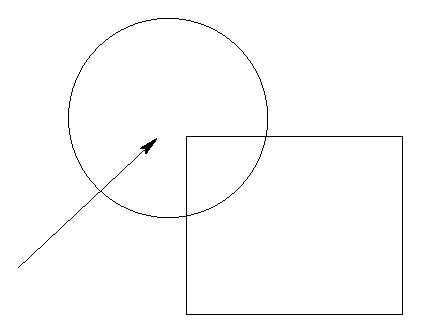
\includegraphics{chapters/chapter1/figures/fig1}}
	\caption[A short caption, for the figure list]{A long caption, for under the figure.}
	\label{fig:fig1}
\end{figure}
You may include figures, such as Figure~\ref{fig:fig1}. Note the short caption has no period at the end of it, while the long caption does (in other words, always provide the short caption without the period, even if the text is the same as the long caption). We recommend using Xfig (which is an open source tool) if you can for your diagrams. Make sure that the files you create are in encapsulated postscript (eps) format. Note that you must not specify the file extension when including the image (this is because PDF generation automatically converts eps image files to PDF files).

\begin{graph}
	\centering{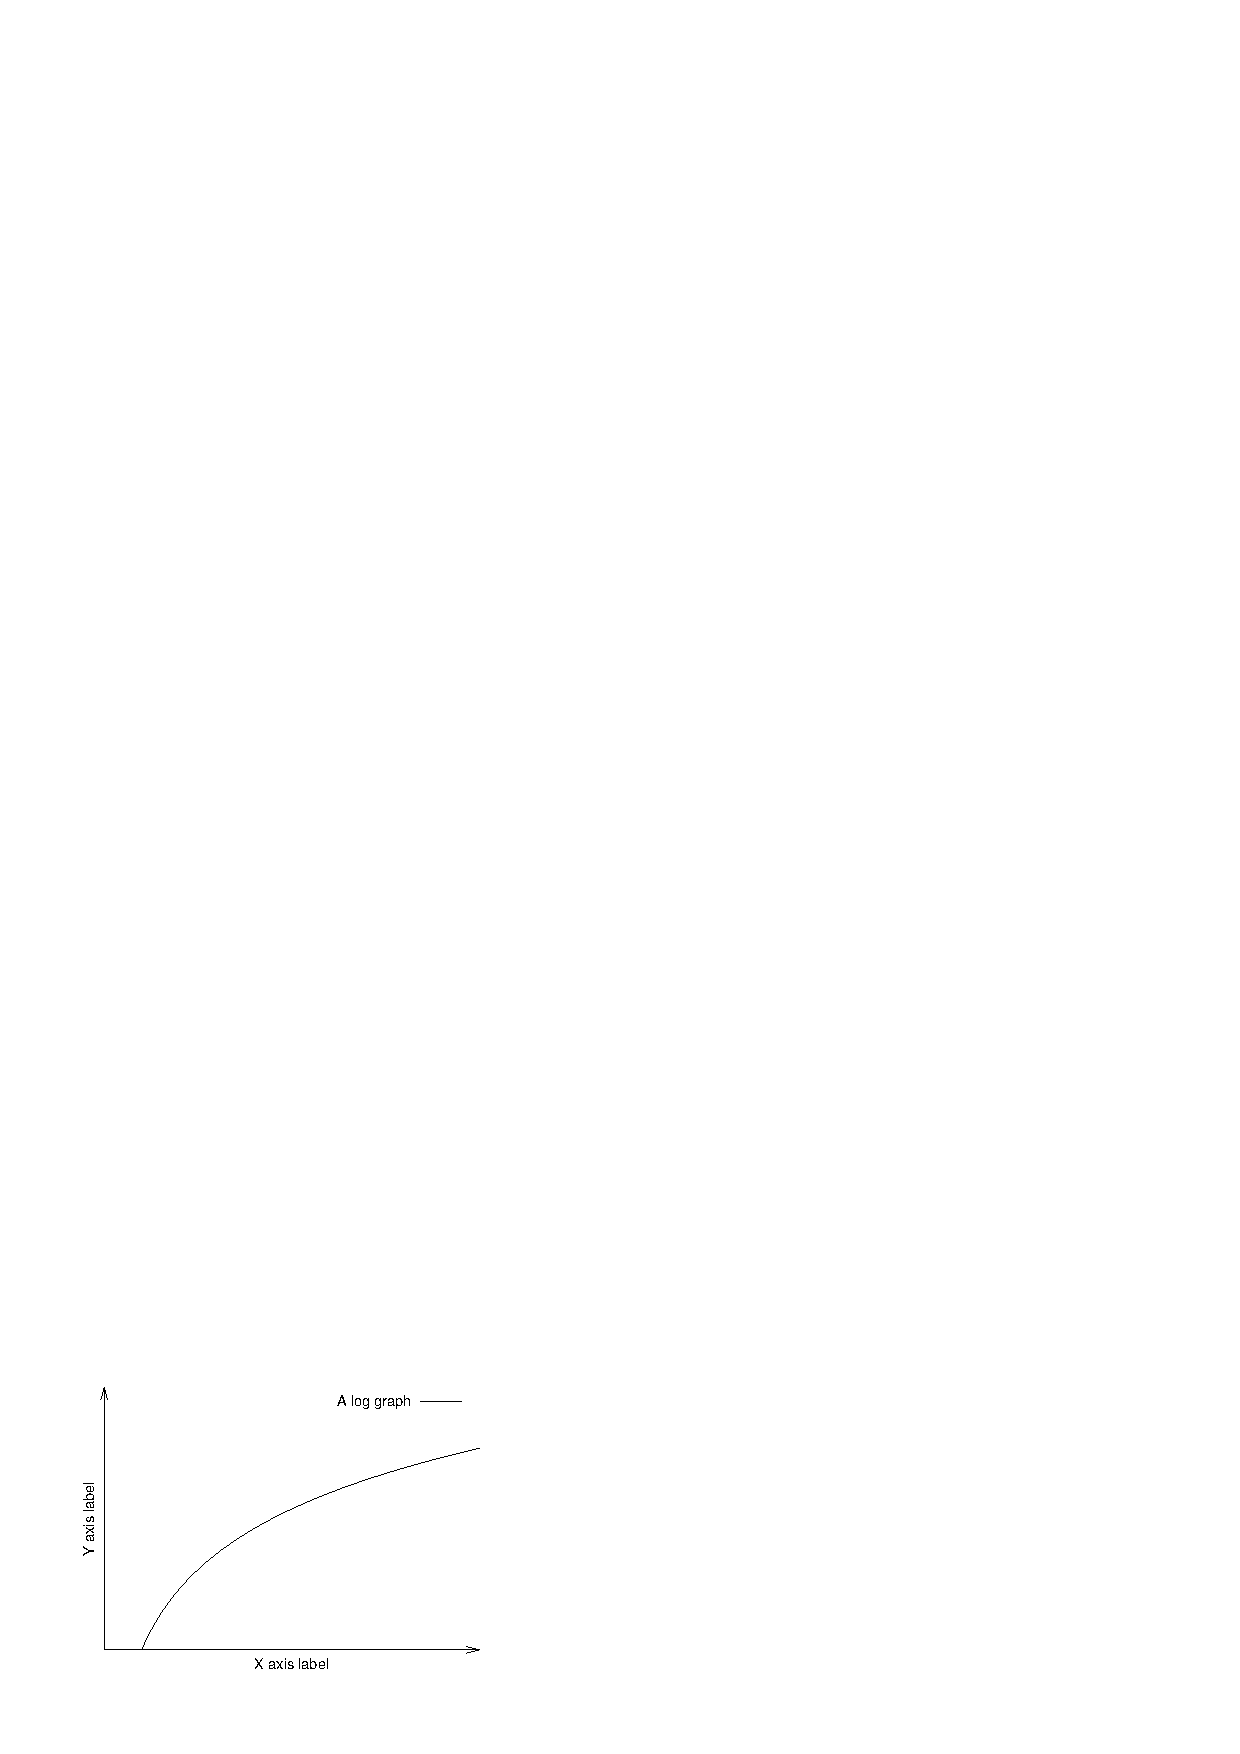
\includegraphics{chapters/chapter1/graphs/graph1}}
	\vspace{10pt}
	\caption[A short graph caption]{A long graph caption.}
	\label{grf:graph1}
\end{graph}
You may also provide graphs, such as Graph~\ref{grf:graph1}. The captions follow the same principal as for figures. We recommend using the very flexible gnuplot (which is open source software) to generate your graphs.

\begin{table}
	\caption[A short table caption]{A long table caption.}
	\centering{
		\begin{tabular}[t]{|l|c|c|}
			\hline
			\textbf{Parameter} & \textbf{Symbol} & \textbf{Domain}    \\
			\hline
			First           & $A$          & $[2,\infty)$    \\
			Second          & $B$    & $[0.0,\infty)$  \\
			Third           & $C$   & $(0.0,\infty)$  \\
		\end{tabular}
	}
	\label{tab:table1}
\end{table}
You may include tables, such as Table~\ref{tab:table1}. The captions follow the same principal as for figures and graphs. You may use a package called \texttt{hhline} to add fancy borders to your tables. Please refer to the package documentation for details.

\begin{algorithm}
	\centering{\fbox{\parbox[]{155mm}{
		\setlength{\parindent}{0.3cm}
		\vspace{0.3cm}
		\small{
		\indent Initialise all variables
		\par\textbf{repeat:}
		\par\hspace{1cm}Select a pattern, and load it
		\par\hspace{1cm}\textbf{for all} {\em values $v$ in the pattern\/} \textbf{do}
		\par\hspace{1cm}\hspace{1cm}Analyse the pattern
		\par\hspace{1cm}\textbf{end for}
		\par\textbf{until} {\em stopping criteria are met}
		}
		\vspace{0.3cm}
	}}}
	\caption[A short algorithm caption]{A long algorithm caption.}
	\label{alg:algorithm1}
\end{algorithm}
Finally, you may add algorithms, such as Algorithm~\ref{alg:algorithm1}. You are free to typeset these as you see fit, or use one of the many algorithm-related packages that are available. In the future, we will try to develop a nice way of generating pseudocode in a standard format like what you see in Algorithm~\ref{alg:algorithm1}. Again, the captioning conventions are the same as for figures, graphs and tables.

All floating bodies (i.e.\ figures, graphs, tables and algorithms) are automatically positioned by \LaTeX. You can change this behaviour by modifying a number of fractions that govern when and where \LaTeX\ can position floating bodies. These are located in \texttt{dissertation.tex}, and there are a several you can modify (e.g.\ \texttt{topfraction}, \texttt{bottomfraction}, \texttt{textfraction} and \texttt{floatpagefraction}). Note that any floating bodies that cannot be placed throughout the text will group together on ``float pages''.

%%%%%%%%%%%%%%%%%%%%%%%%%%%%%%%%%%%%%%%%%%%%%%%%%
%%%%%%%%%%%%%%%%%%%%%%%%%%%%%%%%%%%%%%%%%%%%%%%%%

\section{A Second Section}
\label{sec:first:second_sec}

This is how a second section would appear in your document. You cannot nest sections in one another (to get that effect, use sub-section). It may improve the flow of your writing if you introduce the subsections before jumping into them, so that the reader has an idea of what is coming. Again, use the subsection's labels to ensure that the correct numbering is used throughout.

%%%%%%%%%%%%%%%%%%%%%%%%%%%%%%%%%%%%%%%%%%%%%%%%%

\subsection{A Subsection}
\label{sec:first:second_sec:sub}

You may place subsections as well. Again, these cannot be nested in one another. Consider the overall structure of your dissertation very carefully before writing. Try to avoid too many short subsections, and split your discussion logically between sections and subsections.

\subsubsection{A Sub-Subsection}
\label{sec:first:second_sec:sub:subsub}

You may even add a third level of headings, called sub-subsections (although these are not numbered, or listed on the contents page). It pays to carefully consider whether you will be including sub-subsections. If the text for such a section is short, and there aren't many topics to cover, bulleted lists often look better. However, if the text needs to be broken up into paragraphs, rather use sub-subsections. Also, try to avoid too many sub-subsections, since they cannot be referenced properly, and may become confusing to the reader if they stretch over too many pages. Also, note that while you can label a sub-subsection (just like a section or subsection), referencing the label will simply provide the number of the subsection within which the sub-subsection is located.

You can include acronyms in your dissertation as follows: \useacronym{AI}, \useacronym{ANN} and \useacronym{CI}. The acronyms should all be defined in \texttt{dissertation.tex}, using \texttt{newacronym}. Note that on the first use of the acronym, the full term is used, with the acronym following it in parentheses. On subsequent uses (such as \useacronym{AI}), only the acronym is given.

While it is not at all necessary, you might like to include index terms in your dissertation. You can do this by providing index terms in the text when you mention the topic (e.g.\ widgets\index{Widgets}). You can make an index term bold in the index if it's a primary page reference (e.g.\ for artificial intelligence\index{Artificial Intelligence|idxbf}). If you index the same term again, it will show up as a non-bold secondary reference. You can provide references to other index terms in the \texttt{dissertation.tex} file. There are many more options, but these are outlined properly in the \texttt{makeindx} documentation.

%%%%%%%%%%%%%%%%%%%%%%%%%%%%%%%%%%%%%%%%%%%%%%%%%
%%%%%%%%%%%%%%%%%%%%%%%%%%%%%%%%%%%%%%%%%%%%%%%%%

\section{Summary}
\label{sec:first:summary}

This section should follow all the previous ones forming the main body of the chapter. Provide an outline of the previous sections of this chapter, explaining what each dealt with. Provide section references using labels, as you did for the outline at the start of the chapter.

Give a brief synopsis of what the following chapter will cover, in a general sense. This will improve the logical flow of your work from one chapter to the next.

%%%%%%%%%%%%%%%%%%%%%%%%%%%%%%%%%%%%%%%%%%%%%%%%%
%%%%%%%%%%%%%%%%%%%%%%%%%%%%%%%%%%%%%%%%%%%%%%%%%